\begin{savequote}[75mm]
Nulla facilisi. In vel sem. Morbi id urna in diam dignissim feugiat. Proin molestie tortor eu velit. Aliquam erat volutpat. Nullam ultrices, diam tempus vulputate egestas, eros pede varius leo.
\qauthor{Quoteauthor Lastname}
\end{savequote}

\chapter{Software for VELO}
(@TODO add why this was needed)

\section{Storck}

Storck stands for \" Data \textbf{Stor}age and Tra\textbf{ck}ing \". It is a database system, created for the purpose of storing Velo calibration data.
It was developed using python and django framework.
(@TODO too reference that)
Ath the time of writing, it is being adapted ad CERN for use in the comissioning of VELO.
This section will present it's design.
The details of the implementation can be reffered to in the CERN's gitlab repository link in the bibiliography \cite{bworld}

\subsection{Motivation}

The Scientific workflow when preparing or managing a high energy particle detector requires taking vast ammounts of different types of data. Apart from the immidiate data coming from the device other data types, such as conditions of the test or the detector (such as temperature, date, duration of the test) are needed as well. 
The developement process might be messy, and evolve in time. This is also true for the monitoring tasks when using the detector for taking measurements. 
On the other hand, relational databases require predefined structure, that is not easy to be modified when the data have been filled. 
Relational and non-relational databases tend to be not the best solution when used to store binary files.
For those reasons, the Storck project was created.
It utilises relational database with non-relational elements with filesystem storage.
It is not oriented towards a one type of files, nor does it expect any kind of predefined structure.
Storck allows to share data between it's users, and track the changes in the data.


\subsection{Software Technology}

\subsubsection{Django and Django rest api}
Python language provides many web frameworks.
One of the most popular of them is Django. 
(@TODO add reference to website https://www.djangoproject.com/)
Django is mature web design framework, based on the Model-View-Controller (MVC) design pattern. Django is splitted between Model, View and Template, thoigh
tt's important to note that functionally Django View corresponds to Controller, and Template to View parts of MVC.
This design pattern allows for logical separation the functional responsibility of the code.
Furtherly, Django's design consist of apps. Each of the apps implements their own version of MVC, though it is possible to use any of the component of the MVC design from any other app.
This framework also utilises object–relational mapping, which is freeing the framework user from writing queries using SQL language, and allows for high level object oriented usage of the model.

\subsubsection{PostgresSQL}
PostgresSQL is popular implementation of relational database. It is SQL compliant. Importantly, it also has non-relational capability. It i

\subsubsection{Docker}

Docker provides OS-level virtualisation. It uses images and containers. Docker image is a software package that contains everything that is necessarry to run an app.
Images are defined in special files called Dockerfiles. Image definition is done by using Dockerfile commands.
Images are usually based on operating system's, like Ubuntu Linux or Alpine Linux.
The former is by far the most popular choice, as the base image from alpine linux needs only 8 MB of disk space.
When Images are being mounted to the docker daemon, they are reffered to as containers.

\subsection{Service Design Overview}

The design of the system at heart uses REST API communication for managing the access to the database.
Users have have multiples ways of interacting with Storck; but all of them internally use REST API.
Users can use the web interface, and manually input or download the data.
For the purposes of the ease of use, there also exists a python wrapper to the REST API, so users can easilly create scripts that will interact with Storck.
When the web server receives commands via REST API, it interacts with PostgresSQL in order to validate the request, and responds using HTTP request, either by providing requested information (like list of files, file details) or by sending the file.
Because http servers may be a bottleneck when serving large ammounts of data, we implemented possibility to download the data using direct files access.
When storing files, storck doesnt write them directly to the database, but it saves it on the disk.
By the design of the CERN's computing ecosystem, this disk space is accessible by ssh connection with the CERN's lxplus servers.
The Fig. \ref{fig:storck_diagram} contains schematic diagram for the data flow in the Storck.


\begin{figure}[H]
\centering
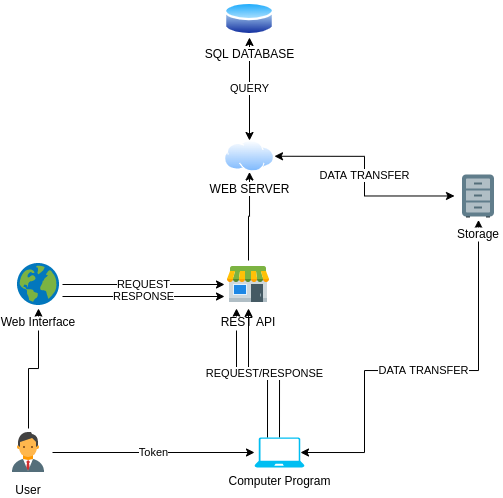
\includegraphics[width=0.7\textwidth]{figures/chapter5/storck/storck diagram.drawio.png}
\caption{
}
\label{fig:storck_diagram}
\end{figure}

\subsection{Implementation}

The overall implementation spans over a few django apps. We will not present here parts of the code, as we feel this would be excessive.
Yet we provide an overview over the most important parts of the implementation of the service

\subsubsection{Files}

\begin{table}[h]
\begin{center}
\begin{tabular}{ |c|c| }
\hline
Property & Django model type \\
\hline
id & AutoField \\
file & FileField \\
hash & TextField \\
workspace & ForeignKey \\
user & ForeignKey \\
previous\_version & ForeignKey \\
duplicate\_of & ForeignKey \\
date & DateTimeField \\
fake\_path & TextField \\
meta\_open & JsonField \\
meta\_closed & TextField \\
hide & BooleanField \\
\hline
\end{tabular}
\caption{\label{tab:storck_filesfield}Table of contents of the StorckFile model.}
\end{center}
\end{table}

The most important element of the Storck is the StorckFile model/database. It records the files uploaded, and stores proper information.
The \textit{id} field contains an unique id that identifies each of the files in the database.
(@TODO make name cursive)
Next, the file, which is of django's File field type, contains a path to locally saved file.
This property is not implicitly created as the request to file with its contents comes in, but instead it is created with the deduplication procedure described in Sec \ref{deduplication:sec}.
Hash is the md5sum of the contents of the file, calculated upon receiving.
Workspace and user contains a foreign key connection to the list of all workspaces and users.
User field contains user id of the user who uploaded this file (or its duplicate).
previous\_version points to the record containing the previous version of the given file.
Here ``new version'' means a new file in given workspace with the same ``fake\_path'' attribute.
(@TODO check if this is really coverd in the code)
duplicate\_of contains a reference to the files duplicate record.
fake\_path is the logical path of the file. This property has no physical sense for the Storck database, as the files are not stored using this path.
meta\_open is the the metada property. It is JsonField, which makes it flexible, and allows to create arbitrary structure of the data inside of the field.
Because we don't want to show older versions of files in the web view, we use flag hide to decide whether the file is shown or not.


\subsubsection{Authentication}
The CERN's ecosystem allows for authentication of CERN users*. It uses (OIDC) OpenID Connect system, whichi was build on top of OAuth 2.0 framewrok.
OIDC system allows for third-party identification.
(@TODO refernece OIDC, OAuth )
What that means is that instead of requiring a proprietary login password in Storck, we can use redirect the login to CERN SSO (CERN single sign on) service.
There, user can use their CERN Account password and login, the same that is being used for other services at CERN to log in.
Automatically, in the background, CERN SSO communicates to the web server and confirms the identity of the user.
On the administrator side, setting up the authentication with OIDC requires setting proper tokens. Those can be generated using the CERN application portal.
Although in the section we refer to CERN's procedures of authentication, for anyone willing to reuse Storck other purposes, it is possible to do that with any authentication system that implements the OIDC.
None of the parts of this process is specifically dedicated only to the CERN ecosystem.

*each person at CERN can use CERN account to authenticate or log in to multiple services.

\subsubsection{Deduplication}
\label{sec:deduplication}

The deduplication process is used when the file is about to be saved in the storck.
The contents of the file must be received by the server, and when they are, server calulates the md5sum hash value.
(@TODO reference the md5sum)
The database is then checked for the hash matching the file.
Is the same hash exists in the database, then the record containig this hash is the duplicate of the incoming file.
If the file has no duplicate, it is processed and saved normally.
But if the duplicate exists, the received file content is discarded.
The entry to the file database is progressed normally, and the file path to the incoming file is set to be the same as for the already existing file.
Addiitonaly the attribute duplicate\_of is also set to point to the id of the entry of the existing file record.

\subsection{REST API}

The REST API makes for a perfect interface for project like this.
(@TODO add reference to REST A{O})
Most of the modern programming languages are capable of making HTTP request be themselves, and network connection is usually necessarry for any operation.
REST API is agnostic of an operating system, and programing language.
In my previous experience with LHCb monitoring, one of the biggest challenges was compatibility of the database tools, which only interfaced by C++ library.
The design of STORCK is free of this problem, as the client of the system doesn't need to update every time there is a change in the Storck service.


\begin{center}
\begin{tabular}{ c c c }
\hline
method & path & params \\
\hline
GET & /api/workspaces &  \\
\hline
POST & /api/workspace & name (body) \\
\hline
POST & /api/workspace/user & workspacetoken (body) \\
 & & userid (body)
 \label{tab:workspace-api}
\end{tabular}
\end{center}


\begin{center}
\begin{tabular}{ c c c }
\hline
method & path & params \\
\hline
GET & /api/files & hidden (query) \\
 & & token (query) \\
\hline
 GET & /api/file & info (query) \\
 & & id (query) \\
 & & token (query) \\
\hline
 POST & /api/file & token (query) \\
 & & file (body) \\
 & & path (body) \\
 & & meta (body)
  \label{tab:file-api}
\end{tabular}
\end{center}

(@TODO consult this subsection with the code)
The Tab. {tab:workspace-api}, {tab:file-api}, present the listing of the REST API methods.

The rest API consists of two endpoints

\subsection{Deployment}

The novel deployment process standard in the IT industry is using Dockerisation.
And so, Storck in it's deployment depends on it.

\begin{figure}[H]
\centering
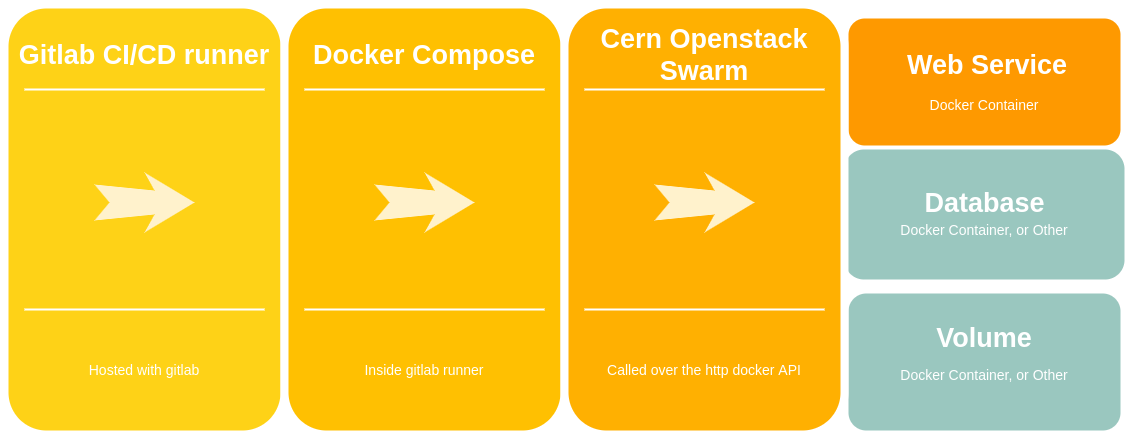
\includegraphics[width=0.7\textwidth]{figures/chapter5/storck/storck_dockers.drawio.png}
\caption{The schematic of Storck deployment process. The light green color means optional components.}
\label{fig:storck-dockers}
\end{figure}

The Fig. \ref{fig:storck-dockers} depicts the flow of the deployment for storck.
The lowest level of the deployment consists of 3 docker images, Web App, Database and Volume.
The last two are optional as in fact, it is possible to use external (not dockerised) Volume, and external Database service.
Database can be runned simply using a predefined docker image.
Web App is creating using custom Dockerfile. The base image is the Alpine Linux image with python 3.8.
During build of the image, it set's up necessary environment variables, dependencies, migrations, and in the end, runs the uwsgi server.
(@TODO reference uwsgi server)

\subsection{Gitlab CI}

As visible in the Fig. \ref{fig:storck-dockers}, the Gitlab CI running environemnt is the first part of the deployment process.
Although gitlab started purey as a service that allows for hosting and browsing the git repositories, like many other git services, it provides mechanism for Continous Integration / Continuous Deployment.
What it means is that ther is no longer a need for a dedicated server that will be running test environment, and a manuall triggering of some deplyment or testing jobs.
It is now perfectly possible to do those things from the gitlab web interface.

\begin{figure}[H]
\centering
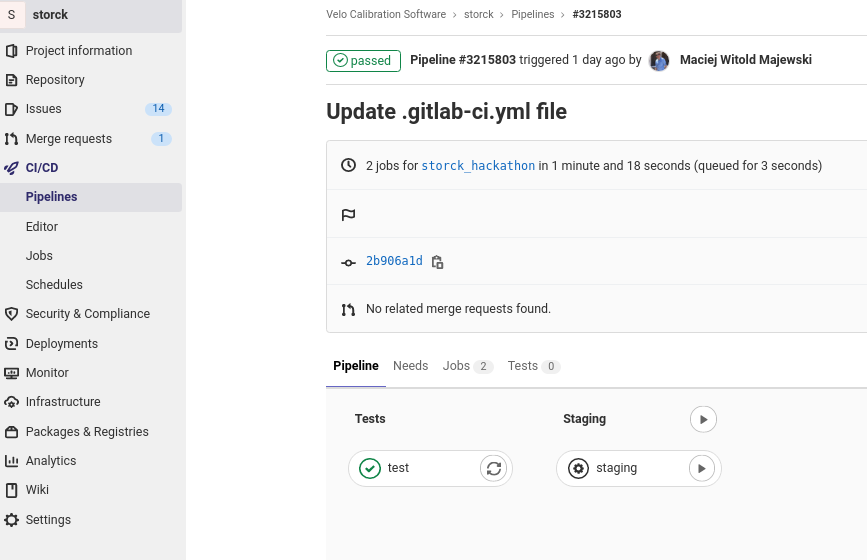
\includegraphics[width=0.7\textwidth]{figures/chapter5/storck/storck_gitlab.png}
\caption{view of a gitlab pipeline}
\label{fig:storck-gitlab}
\end{figure}

Automatic deployment can be set in various ways.
In case of Storck, the pipeline it was set up so that it would run unit tests on every git commit pushed to any branch on gitlab.
Then, if the test did not fail, it is possible to use a button to deploy Storck to staging server.
Only on the master branch, after succesfull deployment of staging it is possible to deploy to the production server.
Fig. \ref{fig:storck-gitlab} shows a view of a single pipeline in gitlab.

\subsection{Storck web interface}

\begin{figure}[H]
\centering
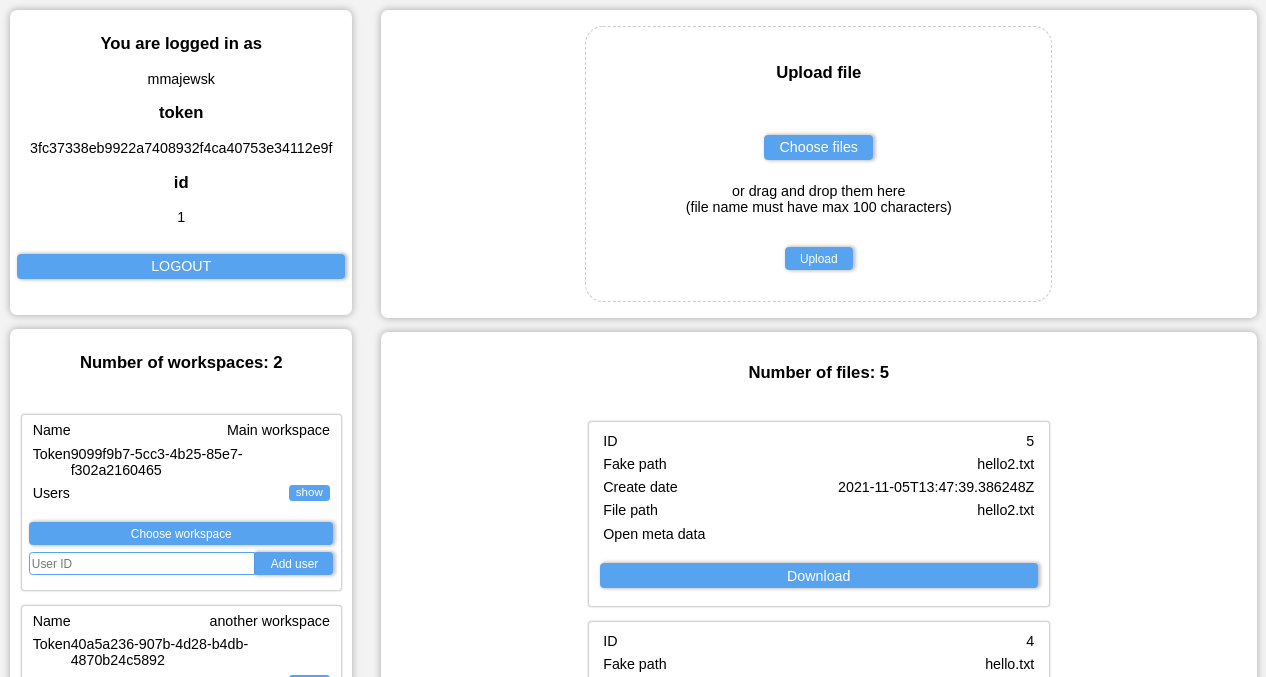
\includegraphics[width=0.7\textwidth]{figures/chapter5/storck/screenshot_web.png}
\caption{Storcks web interface.}
\label{fig:storck-web-interface}
\end{figure}

(@TODO maybe add more in the description)

Storcks web interface is very basic, as it is not meant to be the main way of interacting with storck.
In the Fig. \ref{fig:storck-web-interface}, on the left side there is a space that contains users username, id and user token.
Below that space there is a list of avialible workspaces.
Each of the workspaces shows it's workspace token, and also allows to add users to the workspace.
The two areas on the right side of the screen are devoted to files.
The top area can be used as drag-and-drop area for the files to be uploaded to storck.
The lower area lists all of the fiels contained in the workspace, and button for downloading.


\subsection{Storck python client}

Storck python client was created as a separated project and repository to the main storck project.
To use it, python users can simply install it as a package using a command pip install git+https://gitlab.cern.ch/velo-calibration-software/storck
(@TODO make this install line look better).
It is a very small and simple package.
The very basic usage is as follows:

from storck client import StorckClient

client = StorckClinet(api\_host=..., user\_token=..., workspace\_token=...)
print(client.get\_files())

(@TODO ) ake it a code snippet

The StorckClient class can be used to make an instance of the client. It accepts three arguments, which are as follows: the http adress to storck server, user token and workspace token.
Thise are optional as instead an environmental variable can be used.
The client has several methods which we present in form of a table.
For a more detailed description of all of the methods we refer the reader to the source code.


\begin{table}[h]
\begin{center}
\begin{tabular}{ |c|c| }
\hline
Method & description \\
\hline

auth\_verify & verifies if the credentials are correct\\
set\_workspace_token & sets the workspace token for the object\\
create_workspace & creates new workspace\\
get\_files & outputs list of files currently present in the workspace\\
get\_file & returns all information about given file\\
upload\_file & uploads the contents of the file and its information\\
download\_file & downloads the contents of the file\\
add_user\_to_workspace & adds user to workspace\\
\hline
\end{tabular}
\caption{\label{tab:storck_client}Table of available methods of storck client}
\end{center}
\end{table}

\section{Titania}

Titania is a monitoring framework built with python, Qt and flask.
(@TODO refernce those)
As well as Storck it is being adapted at the Velo group for the purposes of the next runs at LHCb.
This sections will present the design and examplary uses of the framework.


\subsection{Motivation}
Drawing from the experience of working with monitoring in Run 1 and Run 2, we have proposed a new project for handling the monitoring tasks.
The previous software for the monitoring, although useful, was getting difficult in the developement due to the ammounts of different uncoordinated changes.
The source code of the platform was not well structured, so adding new plots was usually quite the challenge.
This is what drove us to developing a new platform for monitoring VELO as a python framework.

\subsection{Software Technology}

Python is one of the most popular tools for plotting and visualistaion in the scientific community.
Famously, the first image of the black hole was created with python, and even in the footage from the first flight on mars the use of matplotlib can be seen.
(@TODO check and reference the sources)
Titania was designed with the desktop GUI in mind first (it also contains some web interface capabilities).
So naturally, we used the PyQt library, which interfaces the QtGUI library to python.
QtGUI in short provides easy way to create cross-platform GUI applications.
It is object oriented library, and impements system of sockets and connections (@TODO check if correct words are used)

\subsection{Framework Design}

As previously stated, one of the key goals of the new system is extensibility, and orderliness.
Inspired by django's concept of implementing MVC in the framework, we define a 3 key components to any monitoring tasks

\begin{enumerate}
  \item Data
  \item Plots
  \item Exploration
\end{enumerate}

Those are a fundamental blocks of any monitoring tasks.


\textbf{Data} here is understood in terms of source of data. Anytime we wan't to show some data we need to access them.
There is multitude of eays that this can be done; reading files from a disk, reading a stream of data, receiving data as http request and others.
This also means a format of the data. Data can be text file of csv structure, binary file, image or sound recording.

\textbf{Plots} are the graphical representation of the data. This means linear plots, or scatter or histogram and others. Each of the ways of f representing the data has it's own custom options of placement and colours and other things.

\textbf{Exploration} - one must be able to choose between diferent data source, and different plot types. If a monitoring service shows only one plot from a one data file, it can hardly be a system.


\subsection{API}
\subsubsection{Data}
\subsubsection{Plots}
\subsubsection{Exploration}
\subsubsection{Views}
\subsubsection{QtGUI - desktop app}
\subsubsection{Web app}
\subsection{Implementation}

\section{Conclusions}


%%% Local Variables:
%%% mode: latex
%%% TeX-master: "../dissertation"
%%% End:
